\documentclass[a4paper,12pt]{article}
\usepackage{cmap}
\usepackage[T2A]{fontenc}
\usepackage[utf8]{inputenc}
\usepackage[english,russian]{babel}
\usepackage{listings}
\usepackage{amsmath}
\usepackage{amsfonts}
\usepackage{float}
\usepackage{csquotes}
\usepackage{graphicx}
\usepackage{hyphenat}
\usepackage{xcolor}
\usepackage{hyperref}
\usepackage{mathtools}
\usepackage{upgreek}


\renewcommand{\theequation}{\thesection.\arabic{equation}}


\author{Шерепа Никита}
\title{ThinkDSP. Лабораторная 9. Дифференцирование и интегрирование.}
\date{\today}

\graphicspath{{res/screenshots}}

\begin{document}%
	
	\maketitle
	
	\newpage \tableofcontents
	\newpage \listoffigures
	\newpage \lstlistoflistings
	
	\newpage
	
	\definecolor{dkgreen}{rgb}{0,0.6,0}
	\definecolor{gray}{rgb}{0.5,0.5,0.5}
	\definecolor{mauve}{rgb}{0.58,0,0.82}
	
	\lstset{
		language=Python,                 % выбор ЯП для подсветки 
		basicstyle=\small\sffamily, % размер и начертание шрифта для подсветки кода
		numbers=left,               % где поставить нумерацию строк (слева\справа)
		numberstyle=\tiny,           % размер шрифта для номеров строк
		stepnumber=1,                   % размер шага между двумя номерами строк
		numbersep=5pt,                % как далеко отстоят номера строк от подсвечиваемого кода
		aboveskip=3mm,
		belowskip=3mm,
		showstringspaces=false,
		columns=flexible,
		captionpos=b, 
		basicstyle={\small\ttfamily},
		numbers=left,
		numberstyle=\tiny\color{gray},
		keywordstyle=\color{blue},
		commentstyle=\color{mauve},
		stringstyle=\color{dkgreen},
		breaklines=true,
		breakatwhitespace=true,
		tabsize=3
	}

	
	\section{Упражнение 9.2}
	
	\begin{enumerate}
		
		\item{Задание}
		
		Создайте треугольный сигнал и напечатайте его. Примените \texttt{diff} к сигналу и напечатайте результат. Вычислите спектр треугольного сигнала, примените \texttt{differentiate} и напечатайте результат. Преобразуйте спектр обратно в сигнал и напечатайте его. Есть ли различия в воздействии \texttt{diff} и \texttt{differentiate} на этот сигнал?
		
		\item{Ход работы}
		
		Создадим треугольный сигнал
		\begin{lstlisting}[caption=Создаем треугольный сигнал]
			in_wave = TriangleSignal(freq=50).make_wave(duration=0.1, framerate=44100)
			in_wave.plot()
			decorate(xlabel='Time (s)')
		\end{lstlisting}
		\begin{figure}[H]
			\centering
			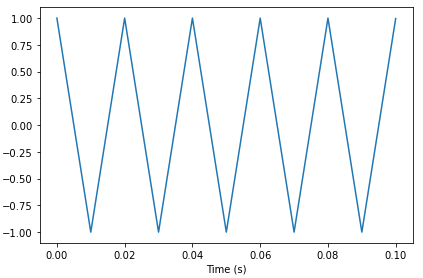
\includegraphics[width=0.75\textwidth]{2_1.png}
			\caption{Треугольный сигнал}
			\label{fig:2.1}
		\end{figure}
		
		Теперь применим в нему \texttt{diff}
		\begin{lstlisting}[caption=Применяем \texttt{diff}]
			out_wave = in_wave.diff()
			out_wave.plot()
			decorate(xlabel='Time (s)')
		\end{lstlisting}
		\begin{figure}[H]
			\centering
			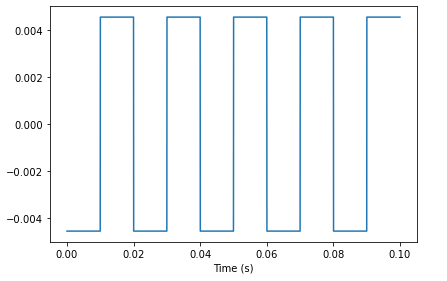
\includegraphics[width=0.75\textwidth]{2_2.png}
			\caption{Сигнал с применением \texttt{diff}}
			\label{fig:2.2}
		\end{figure}
		
		Видим, что получилась прямоугольная волна, что объясняет, почему гармоники в прямоугольной волне уменьшаются как $1/f$, по сравнению с треугольной волной, которая спадает как $1/f2$.
		
		
		Теперь вычислим спектр треугольного сигнала и применим \texttt{differentiate}
		\begin{lstlisting}[caption=Спектр сигнала + \texttt{differentiate}]
			out_wave2 = in_wave.make_spectrum().differentiate().make_wave()
			out_wave2.plot()
			decorate(xlabel='Time (s)')
		\end{lstlisting}
		\begin{figure}[H]
			\centering
			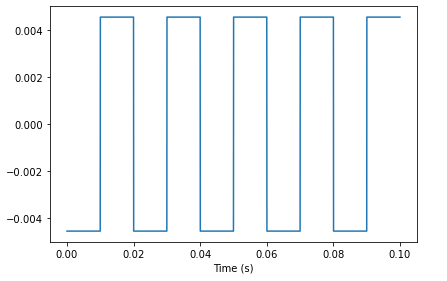
\includegraphics[width=0.75\textwidth]{2_2.png}
			\caption{Спектр сигнала + \texttt{differentiate}}
			\label{fig:2.2}
		\end{figure}
		
		Когда мы берём спектральную производную, то получаем "звон" вокруг разрывов.
		
		Различия между \texttt{diff} и \texttt{differentiate} в том, что производная треугольной волны не определена в точках треугольника.
		
	\end{enumerate}
	\newpage
	
	\section{Упражнение 9.3}
	
	\begin{enumerate}
		
		\item{Задание}
		
		Создайте прямоугольный сигнал и напечатайте его. Примените \texttt{cumsum} и напечатайте результат. Вычислие спектр прямоугольного сигнала, примените \texttt{integrate} и напечатайте результат. Преобразуйте спектр обратно в сигнал и напечатайте его. Есть ли различия в воздействии \texttt{cumsum} и \texttt{integrate} на этот сигнал?
		
		\item{Ход работы}
		
		Создадим прямоугольный сигнал
		\begin{lstlisting}[caption=Создаем прямоугольный сигнал]
			in_wave = SquareSignal(freq=50).make_wave(duration=0.1, framerate=44100)
			in_wave.plot()
			decorate(xlabel='Time (s)')
		\end{lstlisting}
		\begin{figure}[H]
			\centering
			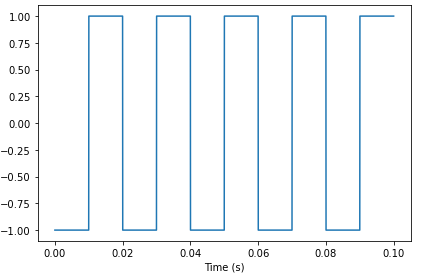
\includegraphics[width=0.75\textwidth]{3_1.png}
			\caption{Треугольный сигнал}
			\label{fig:3.1}
		\end{figure}
		
		Теперь применим в нему \texttt{cumsum}
		\begin{lstlisting}[caption=Применяем \texttt{cumsum}]
			out_wave = in_wave.diff()
			out_wave.plot()
			decorate(xlabel='Time (s)')
		\end{lstlisting}
		\begin{figure}[H]
			\centering
			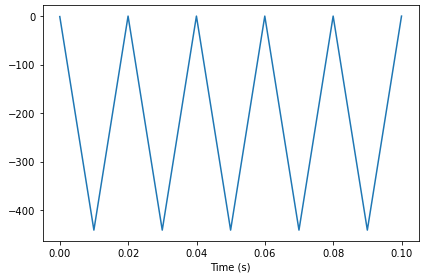
\includegraphics[width=0.75\textwidth]{3_2.png}
			\caption{Сигнал с применением \texttt{cumsum}}
			\label{fig:3.2}
		\end{figure}
		
		Видим, что получилась треугольная волна. По сути, мы сделали полностью противоположную операцию той, которая была в прошлом упражнении.
		
		
		Теперь вычислим спектр треугольного сигнала и применим \texttt{integrate}
		\begin{lstlisting}[caption=Спектр сигнала + \texttt{integrate}]
			spectrum = in_wave.make_spectrum().integrate()
			spectrum.hs[0] = 0
			out_wave2 = spectrum.make_wave()
			out_wave2.plot()
			decorate(xlabel='Time (s)')
		\end{lstlisting}
		\begin{figure}[H]
			\centering
			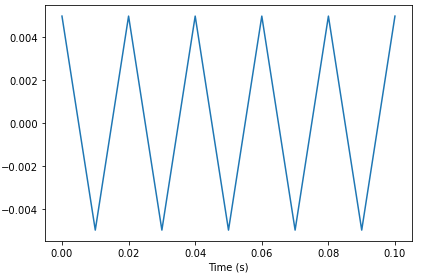
\includegraphics[width=0.75\textwidth]{3_3.png}
			\caption{Спектр сигнала + \texttt{integrate}}
			\label{fig:3.4}
		\end{figure}
		
		Теперь сравним результаты \texttt{cumsum} и \texttt{integrate}.
		\begin{lstlisting}[caption=Сравниваем результаты \texttt{cumsum} и \texttt{integrate}]
			out_wave.unbias()
			out_wave.normalize()
			out_wave2.normalize()
			out_wave.plot()
			out_wave2.plot()
			
			out_wave.max_diff(out_wave2)
			
			Output
			0.0045351473922902175
		\end{lstlisting}
		\begin{figure}[H]
			\centering
			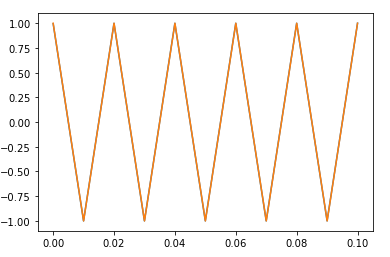
\includegraphics[width=0.75\textwidth]{3_4.png}
			\caption{Сравниваем результаты \texttt{cumsum} и \texttt{integrate}}
			\label{fig:3.4}
		\end{figure}
		
		Видим, что разница = 0.0045351473922902175, т.е отличий между \texttt{cumsum} и \texttt{integrate} почти нет.
		
	\end{enumerate}
	\newpage
	
	\section{Упражнение 9.4}
	
	\begin{enumerate}
		
		\item{Задание}
		
		Создайте пилообразный сигнал, вычислите его спектр, а затем дважды примените \texttt{integrate}. Напечатайте результирующий сигнал и его спектр. Какова математическая форма сигнала? Почему он напоминает синусоиду?
		
		\item{Ход работы}
		
		Создадим пилообразный сигнал
		\begin{lstlisting}[caption=Создаем пилообразный сигнал]
			in_wave = SawtoothSignal(freq=50).make_wave(duration=0.1, framerate=44100)
			in_wave.plot()
			decorate(xlabel='Time (s)')
		\end{lstlisting}
		\begin{figure}[H]
			\centering
			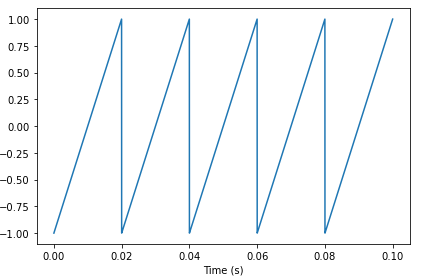
\includegraphics[width=0.75\textwidth]{4_1.png}
			\caption{Пилообразный сигнал}
			\label{fig:4.1}
		\end{figure}
		
		Для начала два раза применим \texttt{cumsum}
		\begin{lstlisting}[caption=1ое применение \texttt{cumsum}]
			out_wave = in_wave.cumsum()
			out_wave.unbias()
			out_wave.plot()
			decorate(xlabel='Time (s)')
		\end{lstlisting}
		\begin{figure}[H]
			\centering
			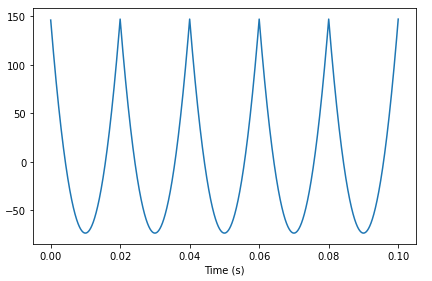
\includegraphics[width=0.75\textwidth]{4_2.png}
			\caption{1ое применение \texttt{cumsum}}
			\label{fig:4.2}
		\end{figure}
		\begin{lstlisting}[caption=2ое применение \texttt{cumsum}]
			out_wave = out_wave.cumsum()
			out_wave.plot()
			decorate(xlabel='Time (s)')
		\end{lstlisting}
		\begin{figure}[H]
			\centering
			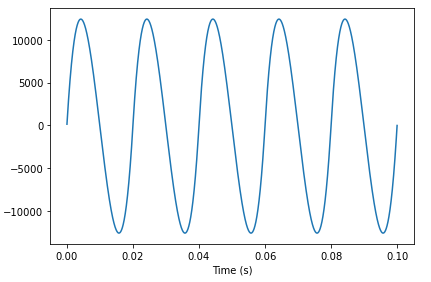
\includegraphics[width=0.75\textwidth]{4_3.png}
			\caption{2ое применение \texttt{cumsum}}
			\label{fig:4.3}
		\end{figure}
		
		После первого применения получили параболу, а после второго - кубическую кривую
		
		Теперь дважды применим \texttt{integrate}
		\begin{lstlisting}[caption=Двойное интегрирование]
			spectrum = in_wave.make_spectrum().integrate().integrate()
			spectrum.hs[0] = 0
			out_wave2 = spectrum.make_wave()
			out_wave2.plot()
			decorate(xlabel='Time (s)')
		\end{lstlisting}
		\begin{figure}[H]
			\centering
			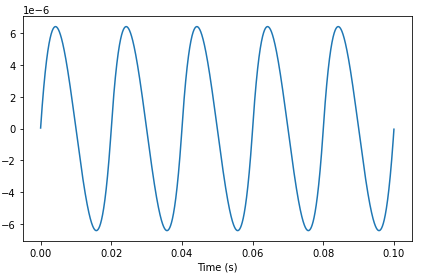
\includegraphics[width=0.75\textwidth]{4_4.png}
			\caption{Двойное интегрирование}
			\label{fig:4.4}
		\end{figure}
	
		Также получили кубическую кривую.
		
		Теперь распечатаем итоговый спектр
		\begin{lstlisting}[caption=Итоговый спектр]
			out_wave2.make_spectrum().plot(high=500)
		\end{lstlisting}
		\begin{figure}[H]
			\centering
			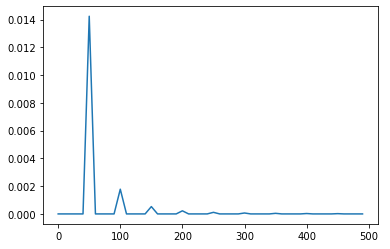
\includegraphics[width=0.75\textwidth]{4_5.png}
			\caption{Итоговый спектр}
			\label{fig:4.5}
		\end{figure}
	
		Результат напоминает синусоиду. Дело в том, что интеграция действует как фильтр нижних частот. И в результате мы отфильтровали почти все, кроме основной частоты.
		
	\end{enumerate}
	\newpage
	
	\section{Упражнение 9.5}
	
	\begin{enumerate}
		
		\item{Задание}
		
		Создайте \texttt{CubicSignal}, определенный в \texttt{thinkdsp}. Вычислите вторую разность, дважды применив \texttt{diff}. Как выглядит результат? Вычислите вторую производную, дважды применив \texttt{differentiate} к спектру. Похожи ли результаты?
		
		Распечатайте фильтры, соответсвующие второй разнице и второй производной, и сравните их.
		
		\item{Ход работы}
		
		Создадим кубический сигнал
		\begin{lstlisting}[caption=Создаем пилообразный сигнал]
			from thinkdsp import CubicSignal
			
			in_wave = CubicSignal(freq=0.0005).make_wave(duration=10000, framerate=1)
			in_wave.plot()
		\end{lstlisting}
		\begin{figure}[H]
			\centering
			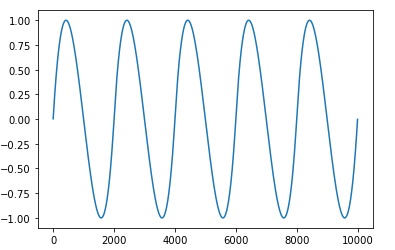
\includegraphics[width=0.75\textwidth]{5_1.png}
			\caption{Кубический сигнал}
			\label{fig:5.1}
		\end{figure}
		
		Дважды применим \texttt{diff}
		\begin{lstlisting}[caption=1ое применение \texttt{diff}]
			out_wave = in_wave.diff()
			out_wave.plot()
		\end{lstlisting}
		\begin{figure}[H]
			\centering
			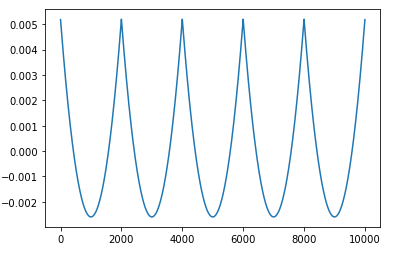
\includegraphics[width=0.75\textwidth]{5_2.png}
			\caption{1ое применение \texttt{diff}}
			\label{fig:5.2}
		\end{figure}
		\begin{lstlisting}[caption=2ое применение \texttt{diff}]
			out_wave = out_wave.diff()
			out_wave.plot()
		\end{lstlisting}
		\begin{figure}[H]
			\centering
			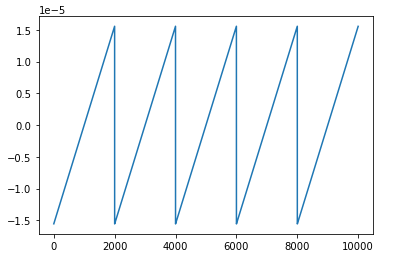
\includegraphics[width=0.75\textwidth]{5_3.png}
			\caption{2ое применение \texttt{diff}}
			\label{fig:5.3}
		\end{figure}
		
		После первого применения получили параболу.
		После второго - пилообразный сигнал.
		
		
		Теперь вычислим вторую производную - дважды применим \texttt{differentiate}
		\begin{lstlisting}[caption=Вычисляем вторую производную]
			spectrum = in_wave.make_spectrum().differentiate().differentiate()
			out_wave2 = spectrum.make_wave()
			out_wave2.plot()
			decorate(xlabel='Time (s)')
		\end{lstlisting}
		\begin{figure}[H]
			\centering
			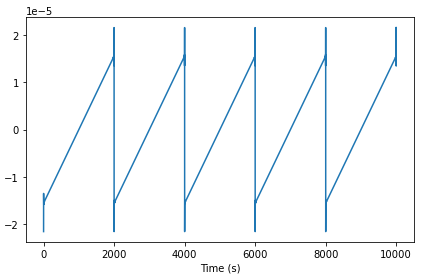
\includegraphics[width=0.75\textwidth]{5_4.png}
			\caption{Вторая производная}
			\label{fig:5.4}
		\end{figure}
		
		В итоге получили пилообразную форму с некоторым "звоном". Проблема в том, что производная параболического сигнала не определена в точках.
		
		Теперь распечатаем фильтр второй разницы: применим ДПФ
		\begin{lstlisting}[caption=Фильтр второй разницы]
			from thinkdsp import zero_pad
			from thinkdsp import Wave
			
			diff_window = np.array([-1.0, 2.0, -1.0])
			padded = zero_pad(diff_window, len(in_wave))
			diff_wave = Wave(padded, framerate=in_wave.framerate)
			diff_filter = diff_wave.make_spectrum()
			diff_filter.plot(label='2nd diff')
			
			decorate(xlabel='Frequency (Hz)',
			ylabel='Amplitude ratio')
		\end{lstlisting}
		\begin{figure}[H]
			\centering
			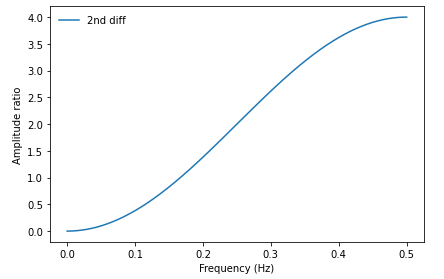
\includegraphics[width=0.75\textwidth]{5_5.png}
			\caption{Фильтр второй разницы}
			\label{fig:5.5}
		\end{figure}
		
		И фильтр второй производной: вычислим филтр первой производной и возведем его в квадрат
		\begin{lstlisting}[caption=Фильтр второй производной]
			PI2 = np.pi * 2
			
			deriv_filter = in_wave.make_spectrum()
			deriv_filter.hs = (PI2 * 1j * deriv_filter.fs)**2
			deriv_filter.plot(label='2nd deriv')
			
			decorate(xlabel='Frequency (Hz)',
			ylabel='Amplitude ratio')
		\end{lstlisting}
		\begin{figure}[H]
			\centering
			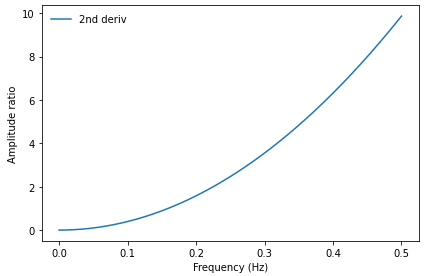
\includegraphics[width=0.75\textwidth]{5_6.png}
			\caption{Фильтр второй производной}
			\label{fig:5.6}
		\end{figure}
		
		Теперь сравним два получившихся фильтра
		\begin{lstlisting}[caption=Сравнение фильтров]
			diff_filter.plot(label='2nd diff')
			deriv_filter.plot(label='2nd deriv')
			
			decorate(xlabel='Frequency (Hz)',
			ylabel='Amplitude ratio')
		\end{lstlisting}
		\begin{figure}[H]
			\centering
			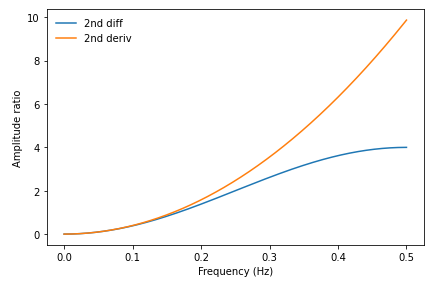
\includegraphics[width=0.75\textwidth]{5_7.png}
			\caption{Сравнение фильтров}
			\label{fig:5.7}
		\end{figure}
		
	
		Видим, что оба являются фильтрами высоких частот, которые усиливают компоненты самых высоких частот. Вторая производная параболическая, поэтому она сильнее всего усиливает самые высокие частоты. Вторая разница - хорошее приближение второй производной только на самых низких частотах, затем она существенно отклоняется.
		
	\end{enumerate}
	\newpage
	
	\section{Вывод}
	
	В результате выполнения лабораторной работы получены навыки работы с
	
	\begin{enumerate} 
		\item \texttt{cumsum} - совокупной суммой
		\item \texttt{integrate} - интегрированием
		\item \texttt{diff} - разницей
		\item \texttt{differentiate} - производными
	\end{enumerate} 
	Также изучены их влиялия на разные типы сигналов.
	
\end{document}
